\documentclass[11pt,a4paper]{report}

\usepackage[margin=2.4cm]{geometry}
\usepackage[T1]{fontenc}
\usepackage[utf8]{inputenc}
\usepackage{lmodern}
\usepackage{amsmath,amssymb,bm}
\usepackage{booktabs,longtable,array}
\usepackage{graphicx}
\usepackage{xcolor}
\usepackage{enumitem}
\usepackage{listings}
\usepackage{hyperref}
\usepackage{caption}
\usepackage{float}

\hypersetup{
  colorlinks=true,
  linkcolor=blue!50!black,
  urlcolor=blue!60!black,
  citecolor=blue!50!black,
  pdftitle={Spectrometer Simulation Project Documentation}
}

\definecolor{codeblue}{RGB}{30,70,150}
\definecolor{codegreen}{RGB}{20,110,60}
\definecolor{codegray}{RGB}{245,245,245}
\lstset{
  language=Python,
  basicstyle=\ttfamily\small,
  keywordstyle=\color{codeblue}\bfseries,
  commentstyle=\color{codegreen},
  backgroundcolor=\color{codegray},
  frame=single,
  breaklines=true,
  showstringspaces=false,
  tabsize=4
}

\newcommand{\code}[1]{\texttt{#1}}
\newcommand{\vect}[1]{\bm{#1}}

\title{Spectrometer Simulation\\Technical and User Documentation}
\author{Final Project Submission}
\date{October 2026}

\begin{document}
\maketitle

\begin{abstract}
This document describes the software architecture, physical model, numerical
methods, configuration, execution workflow, outputs, validation strategy, and
extension points of the spectrometer simulation contained in the
\code{Final} directory.  The software follows relativistic charged particles
through prescribed electric and magnetic fields.  It supports analytic Enge
fringe-field models and numerically calculated fields, several time
integrators, accurate boundary-crossing reconstruction, convergence studies,
energy-conservation studies, and synthetic beam distributions for DLA- and
TNSA-like experiments.

The Boolean blocks in \code{main.py} are intentional experiment switches.
They allow individual studies to be isolated without maintaining several
nearly identical driver files.  They are not interpreted as unreachable or
obsolete code in this documentation.
\end{abstract}

\tableofcontents
\listoftables
\clearpage

\chapter{Project Scope}

\section{Purpose}
The project simulates a charged-particle spectrometer in which particles enter
through a pinhole and propagate under static electric and magnetic fields.
The principal outputs are complete particle trajectories, exit positions,
exit velocities, Lorentz factors, detector-impact distributions, and
convergence or conservation diagnostics.

The implementation is suitable for the following studies:
\begin{itemize}[noitemsep]
  \item single-particle trajectories at prescribed kinetic energies;
  \item comparison of Euler, Runge--Kutta, and Boris integration methods;
  \item comparison of analytic and grid-based fields;
  \item the influence of Enge fringe fields and spectrometer geometry;
  \item angularly divergent monoenergetic beams;
  \item energy-distributed DLA-like beams;
  \item multi-species TNSA-like detector maps;
  \item time-step convergence and kinetic-energy conservation.
\end{itemize}

\section{Model assumptions}
The simulator treats particles as independent test particles.  Their charge
and current do not modify the prescribed fields; therefore space charge,
self-fields, collisions, material interactions, radiation reaction, and
collective plasma effects are outside the current model.  The analytic and
numeric field classes are two-dimensional in the $(x,y)$ plane and return a
three-component vector with a zero $z$ component in the numeric model.

SI units are used internally.  User-facing geometry and trajectory plots use
millimetres, while particle energy is specified in MeV.

\chapter{Directory and Module Structure}

\begin{longtable}{p{0.29\textwidth}p{0.65\textwidth}}
\toprule
File or directory & Responsibility \\
\midrule
\endhead
\code{main.py} & Defines the baseline parameters and contains independently enabled experiment blocks. \\
\code{spectrometer/Experiment.py} & Converts units, calculates the initial relativistic state, time step, computational domain, and derived parameters. \\
\code{spectrometer/integrators.py} & Field selection, geometry termination, exit reconstruction, Euler, RK2, RK4, Boris, and collocated Boris pushers. \\
\code{spectrometer/analitic\_fields.py} & Analytic magnetic and electric Enge fringe-field models. \\
\code{spectrometer/numeric\_fields.py} & Multigrid Laplace solver, scalar potentials, staggered field extraction, linear interpolation, and natural-cubic interpolation. \\
\code{spectrometer/custom\_spline\_2D.py} & Project implementation of one- and two-dimensional natural cubic splines. \\
\code{spectrometer/physics.py} & Relativistic Lorentz acceleration, Boris magnetic rotation, and angular decomposition of velocity. \\
\code{spectrometer/simulators.py} & High-level trajectory, beam, convergence, energy, DLA, and TNSA workflows. \\
\code{spectrometer/geometry.py} & Three-dimensional drawing of the spectrometer, shield, and entrance aperture. \\
\code{spectrometer/plot\_result.py} & Trajectory plotting helper. \\
\code{Figures/} & Saved trajectory, field, convergence, energy, DLA, and TNSA results. \\
\code{Fringe fields/} & Reference literature used for fringe-field modelling. \\
\bottomrule
\end{longtable}

The file \code{fields.py} contains an older analytic-field implementation and
plotting utility.  The active integrator imports the analytic models from
\code{analitic\_fields.py}.

\chapter{Physical Model}

\section{Relativistic equation of motion}
The particle momentum is
\begin{equation}
  \vect{p}=\gamma m\vect{v}, \qquad
  \gamma=\frac{1}{\sqrt{1-|\vect{v}|^2/c^2}},
\end{equation}
and the Lorentz force is
\begin{equation}
  \frac{d\vect{p}}{dt}=q\left(\vect{E}+\vect{v}\times\vect{B}\right).
\end{equation}
The velocity equation implemented by \code{get\_lorentz\_acceleration} is
\begin{equation}
  \frac{d\vect{v}}{dt}=\frac{q}{\gamma m}
  \left[
  \vect{E}+\vect{v}\times\vect{B}
  -\frac{\vect{v}(\vect{E}\cdot\vect{v})}{c^2}
  \right].
\end{equation}
The last term enforces the correct relativistic response to an electric field.

\section{Energy-to-velocity conversion}
The input \code{q\_eng\_MeV} is a three-component vector.  Its norm determines
the kinetic energy, while its direction determines the initial velocity
direction.  For kinetic energy $K$,
\begin{equation}
  |\vect{v}_0|=c\sqrt{1-
  \left(\frac{mc^2}{K+mc^2}\right)^2}.
\end{equation}
Consequently, \code{[0, 3, 0]} represents a 3 MeV particle initially directed
along positive $y$.

\section{Coordinate system and geometry}
The coordinate convention is:
\begin{itemize}[noitemsep]
  \item $x$: spectrometer width;
  \item $y$: longitudinal depth and nominal beam direction;
  \item $z$: spectrometer height.
\end{itemize}
The body occupies $|x|<w/2$, $0<y<d$, and $|z|<h/2$.  Before the entrance
plane, the particle is restricted by the circular pinhole radius in both $x$
and $z$.  A particle is propagated only while it remains inside the relevant
entrance or body limits and continues in the forward direction.

\section{Analytic uniform-field exit solution}
For the restricted uniform-field case, the project provides an analytic exit
position for validation.  With relativistic Larmor radius
\begin{equation}
  R=\left|\frac{\gamma m v_\perp}{qB_x}\right|,
\end{equation}
and vertical displacement $h$, the longitudinal detector coordinate is
\begin{equation}
  y_{\mathrm{exit}}=\sqrt{2Rh-h^2}.
\end{equation}
The corresponding angle is
\begin{equation}
  \theta=\cos^{-1}\left(\frac{R-h}{R}\right),
\end{equation}
and the proper-time-like variable used in the code is
\begin{equation}
  \tau=\frac{\theta m}{qB_x}.
\end{equation}
The transverse displacement, including a uniform electric contribution, is
then evaluated from the initial position, initial relativistic velocity, and
constant acceleration in $\tau$.

\chapter{Field Models}

\section{Analytic Enge fringe fields}
The analytic model uses the Enge function
\begin{equation}
  F(\zeta)=\frac{1}{1+\exp(S(\zeta))},\qquad
  S(\zeta)=a_0+a_1\zeta+a_2\zeta^2+a_3\zeta^3.
\end{equation}
The code forms a complex coordinate from $y+ix$ and obtains two transverse
field components from the real and imaginary parts.  Two coefficient sets are
available through \code{sharp\_edge}.  When \code{yoke=0}, entrance and exit
Enge factors are multiplied; when \code{yoke=1}, only the entrance transition
is used.  Setting \code{fringe=0} selects an abrupt uniform field inside the
device and zero field before the entrance.

\section{Numeric scalar-potential solution}
The numeric model solves a two-dimensional Laplace problem on a rectangular
grid.  \code{MagneticPotential} and \code{ElectricPotential} override the
base boundary conditions to represent pole faces or electrodes.  The solution
algorithm performs:
\begin{enumerate}[noitemsep]
  \item Gauss--Seidel smoothing on the finest grid;
  \item residual calculation with second-order central differences;
  \item restriction of the residual to successively coarser grids;
  \item Gauss--Seidel solution of the correction equation;
  \item bilinear prolongation of corrections toward the fine grid;
  \item boundary-condition restoration and post-smoothing;
  \item repetition until the residual threshold or iteration limit is reached.
\end{enumerate}
Grid dimensions of the form $2^k+1$ are appropriate for repeated coarsening.
The solver prints its final residual and iteration count.

\section{Field extraction on a staggered grid}
The magnetic field is obtained from the magnetic scalar potential $\psi$:
\begin{equation}
  B_x=-\mu_0\frac{\partial\psi}{\partial x},\qquad
  B_y=-\mu_0\frac{\partial\psi}{\partial y}.
\end{equation}
The electric field follows from $\vect{E}=-\nabla\phi$.  Forward differences
place $x$ and $y$ components at different half-grid locations.  This staggered
arrangement is preserved by supplying the appropriate coordinate axis to each
interpolator.

\section{Grid interpolation modes}
The parameter \code{grid\_interpulation} accepts the strings
\code{"Linear"} and \code{"Spline"}.

\subsection{Linear interpolation}
Bilinear interpolation uses the four corners of the containing cell.  It is
inexpensive and continuous, but its first spatial derivatives change abruptly
at cell boundaries.  A high-order time integrator can therefore measure
cell-crossing artefacts rather than its formal time order.

\subsection{Natural cubic spline}
The \code{"Spline"} option uses the project implementation in
\code{custom\_spline\_2D.py}.  It is constructed once from an axis pair and a
field array:
\begin{lstlisting}
spline = NaturalCubicSpline2D(x_axis, y_axis, field)
value = spline(x_particle, y_particle)
\end{lstlisting}
The field array must have shape
\code{(len(y\_axis), len(x\_axis))}.  A scalar query returns one interpolated
component; array-valued coordinates return an array of component values.

For one dimension, the spline solves
\begin{equation}
  A\vect{p}''=\vect{b},
\end{equation}
with natural boundary conditions $p''(x_0)=p''(x_N)=0$.  Each interval is
stored in the same form as the original project derivation:
\begin{align}
S_i(x)={}&\alpha_i(x-x_i)^3+\beta_i(x-x_{i+1})^3\\
         &+\gamma_i(x-x_i)+\eta_i(x-x_{i+1}).
\end{align}
The two-dimensional spline first constructs the four $x$ coefficients for
each row and then splines those coefficients along $y$.  Each cell therefore
stores $4\times4=16$ coefficients.  The coefficient tensor has shape
\begin{equation}
  (N_y-1,4,N_x-1,4).
\end{equation}
Construction is global, but each particle query identifies one cell and
evaluates only its 16 coefficients.  For a large grid the coefficient storage
is approximately sixteen times the storage of one scalar field component.

\chapter{Time Integration and Exit Events}

\section{Available integrators}
\begin{longtable}{p{0.18\textwidth}p{0.12\textwidth}p{0.62\textwidth}}
\toprule
Driver name & Formal order & Description \\
\midrule
\endhead
\code{Euler} & 1 & Explicit first-order update; primarily a baseline and error demonstration. \\
\code{RK2} & 2 & Midpoint Runge--Kutta method with midpoint field evaluation. \\
\code{RK4\_Lin} & 4 in the step & Classical four-stage RK4 followed by linear boundary reconstruction.  Endpoint accuracy can be limited by the event interpolation. \\
\code{RK4\_Herm} & 4 & Classical RK4 followed by cubic Hermite boundary reconstruction using position and velocity at both ends of the final step. \\
\code{Boris} & nominally 2 & Electric half-kick, magnetic rotation, electric half-kick, using fields sampled at the current position. \\
\code{Boris\_Coll} & 2 & Collocated variant that samples fields at a predicted half-step position and uses a centred position update. \\
\bottomrule
\end{longtable}

The code chooses a time step from a magnetic time scale and \code{N\_steps}:
\begin{equation}
  \Delta t=\frac{T_{\mathrm{cyclotron,code}}}{N_{\mathrm{steps}}}.
\end{equation}
Thus increasing \code{N\_steps} refines time while leaving the field grid
unchanged.

\section{Linear exit reconstruction}
\code{\_exect\_exist} calculates a fractional position between the last point
inside and first point outside a boundary.  Position is interpolated linearly.
Velocity magnitude and direction are treated separately before recombination,
which reduces artificial changes of speed in magnetic-only motion.

\section{Cubic Hermite exit reconstruction}
\code{\_hermite\_exit\_crossing} represents the last trajectory segment by
\begin{equation}
  \vect{R}(s)=h_{00}\vect{R}_0+h_{10}\Delta t\vect{v}_0
             +h_{01}\vect{R}_1+h_{11}\Delta t\vect{v}_1,
  \qquad 0\le s\le1,
\end{equation}
where $h_{00}$, $h_{10}$, $h_{01}$, and $h_{11}$ are the standard cubic
Hermite basis functions.  The crossed coordinate is solved by bisection.  The
full exit position is evaluated at the resulting fraction, and the tangent is
obtained by differentiating the Hermite curve.  The final velocity direction
is the normalized tangent; its magnitude is interpolated independently
between the two endpoint speeds.  The exit Lorentz factor is recalculated.

This distinction is essential: RK4 can retain fourth-order endpoint behaviour
only when both the right-hand side and the boundary event are reconstructed
with sufficient smoothness and accuracy.

\chapter{Configuration and Execution}

\section{Software requirements}
The code directly imports:
\begin{itemize}[noitemsep]
  \item Python 3;
  \item NumPy;
  \item Matplotlib;
  \item SciPy;
  \item Joblib.
\end{itemize}
The file \code{spectrometer/pips.txt} additionally mentions \code{ipympl} and
\code{kaleido}, which are useful for interactive or exported plots but are not
central to the trajectory solver.

Example installation:
\begin{lstlisting}[language=bash]
python -m pip install numpy matplotlib scipy joblib ipympl kaleido
\end{lstlisting}

Run from the directory containing \code{main.py}:
\begin{lstlisting}[language=bash]
python main.py
\end{lstlisting}
On Windows, the \code{if __name__ == "__main__":} guard must be preserved
because beam simulations use multiprocessing through Joblib.

\section{Principal parameters}
\begin{longtable}{p{0.25\textwidth}p{0.18\textwidth}p{0.49\textwidth}}
\toprule
Parameter & Units/type & Meaning \\
\midrule
\endhead
\code{height\_mm} & mm & Full spectrometer height in $z$. \\
\code{width\_mm} & mm & Full spectrometer width in $x$. \\
\code{depth\_mm} & mm & Longitudinal length in $y$. \\
\code{shield\_mm} & mm & Entrance shield length. \\
\code{pinhole\_dia\_mm} & mm & Entrance aperture diameter. \\
\code{yoke} & 0 or 1 & Controls geometry and whether the analytic model contains a separate exit fringe. \\
\code{R0\_mm} & three-vector, mm & Initial position $[x_0,y_0,z_0]$. \\
\code{q\_eng\_MeV} & three-vector, MeV & Energy magnitude and initial direction. \\
\code{m\_kg} & kg & Particle rest mass. \\
\code{q\_C} & C & Signed particle charge. \\
\code{Bx0\_T} & T & Nominal magnetic-field amplitude. \\
\code{Ex0\_Vm} & V/m & Nominal electric-field amplitude. \\
\code{fringe} & 0 or 1 & Abrupt field or Enge/numeric fringe field. \\
\code{sharp\_edge} & 0 or 1 & Selects one of the two Enge coefficient sets. \\
\code{solution} & string & \code{"Analitic field"} or \code{"Numeric Field"}. \\
\code{N\_steps} & positive number & Time-resolution denominator. \\
\code{Nx\_p}, \code{Ny\_p} & integers & Potential-grid dimensions, preferably $2^k+1$. \\
\code{grid\_interpulation} & string & \code{"Linear"} or \code{"Spline"}. \\
\bottomrule
\end{longtable}

\section{Experiment switches in main.py}
Each major study is enclosed in an \code{if True:} or \code{if False:} block.
This is an intentional lightweight experiment-selection mechanism:
\begin{itemize}[noitemsep]
  \item set exactly the desired model-initialization block to \code{True};
  \item set the desired experiment block or blocks to \code{True};
  \item leave unrelated experiments at \code{False};
  \item when reproducibility matters, start each block from a deep copy of
        \code{params\_beckup};
  \item remember that several \code{True} blocks execute sequentially and can
        open several figures or change shared parameter objects.
\end{itemize}
They should not be removed merely because static analysis labels them as
constant conditions.

\section{Selecting a numeric spline field}
\begin{lstlisting}
solution = "Numeric Field"
grid_interpulation = "Spline"
Nx_p = 2**7 + 1
Ny_p = 2**7 + 1
\end{lstlisting}
After changing any field-defining parameter, update the experiment and rebuild
the selected field model:
\begin{lstlisting}
params = experiment._update_params(params)
integrator._update_params(params)
integrator._update_solution(integrator.solution)
\end{lstlisting}
The rebuild is important for changes to grid size, domain, field amplitude,
fringe configuration, geometry, or interpolation mode.

\chapter{High-Level Simulation Workflows}

\section{Single and multiple trajectories}
\code{basic\_simulator} accepts an integrator, an integrator name, the
experiment, and either one energy vector or an array of energy vectors.  Each
trajectory is run independently.  Multiple particles use Joblib
multiprocessing.  The return values are nested collections of positions in
millimetres, velocities in metres per second, and Lorentz factors.

\section{Fully analytic mapping}
\code{Fully\_analitic} evaluates the restricted analytic exit relationship
over an energy vector and species arrays.  It is useful as a fast baseline and
as a reference for uniform-field tests.

\section{Convergence tests}
\code{convergence\_test} runs selected integrators over a sequence of
\code{N\_steps}, records exit positions, uses the finest result as a numerical
reference, and fits a line in log--log space.  For a reliable order estimate,
use a geometric refinement series such as
\begin{equation}
  N,\;2N,\;4N,\;8N,\ldots
\end{equation}
and supplement the fit with successive Richardson differences
\begin{equation}
  D_N=|Y_N-Y_{2N}|,\qquad
  p_N=\log_2\left(\frac{D_N}{D_{2N}}\right).
\end{equation}
A single fitted slope can be misleading when errors approach roundoff, cancel,
or alternate because Runge--Kutta stages cross interpolation-cell boundaries.

For a time-convergence study, keep the potential grid and interpolation fixed.
For a spatial-convergence study, make the time error much smaller than the
change caused by grid refinement.  The spline smooths the discrete field and
allows RK4 to express its order, but it does not increase the formal order of
the underlying finite-difference potential solution.

\section{Energy-conservation study}
\code{energy\_vs\_N\_steps\_for\_different\_integrators} compares the final
Lorentz factor with its initial value for several methods and time
resolutions.  Magnetic-only motion provides the clearest conservation test,
because a magnetic force changes direction but performs no work.

\section{Angular and spectral beam models}
\code{Non\_collimataed\_beams} samples azimuthal and elevation angles from
exponential, Gaussian, uniform, or zero-width distributions.  It rotates the
initial velocity and optionally draws a two-dimensional impact histogram.

\code{real\_beams} adds exponential, Gaussian, uniform, DLA gamma-distributed,
or monoenergetic energy sampling.  \code{TNSA} repeats this workflow for
several mass, charge, and characteristic-energy values and combines the
impact positions into one detector map.

For reproducible stochastic plots, set a NumPy random seed before sampling:
\begin{lstlisting}
np.random.seed(12345)
\end{lstlisting}

\chapter{Outputs and Interpretation}

Each trajectory integrator returns
\begin{lstlisting}
R_vec_mm, v_vec_m0s, gamma_vec
\end{lstlisting}
where the final sample is reconstructed on the boundary.  Detector maps use
the final $(x,y)$ coordinates.  Potential and field classes also provide
visualization methods for scalar-potential maps, field magnitude, and
streamlines.

The \code{Figures} directory contains representative results.  The following
figures are included only when the files are available, so the document remains
compilable if figures are moved.

\IfFileExists{Figures/Numeric solutions/Field and potential/Figure_111.png}{
\begin{figure}[H]
  \centering
  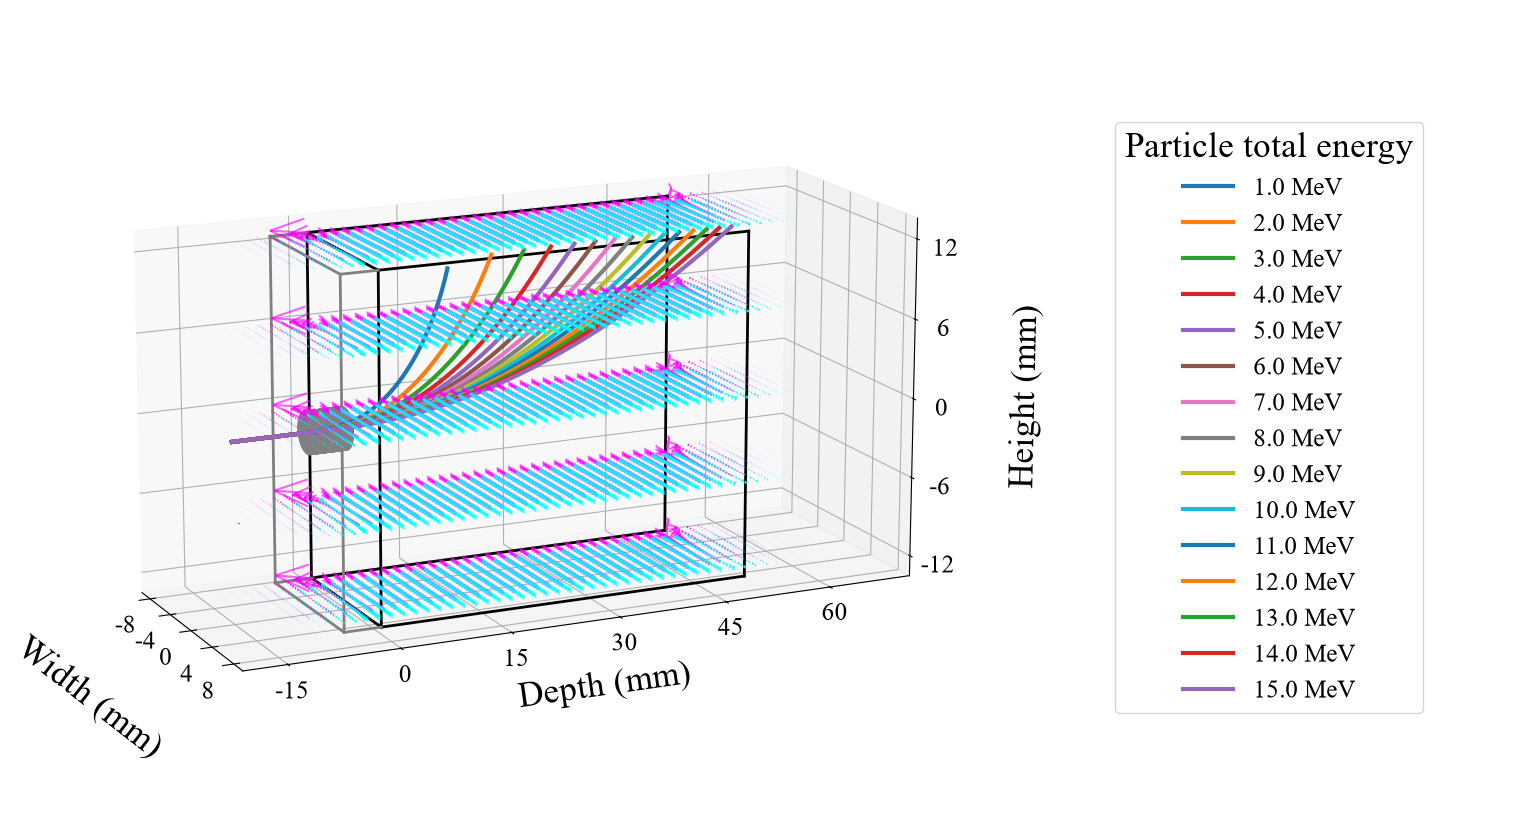
\includegraphics[width=0.82\textwidth]{Figures/Numeric solutions/Field and potential/Figure_111.png}
  \caption{Representative numeric field or potential result stored with the project.}
\end{figure}}{}

\IfFileExists{Figures/Analitic solution/Conversion test/solvers vs analitic.png}{
\begin{figure}[H]
  \centering
  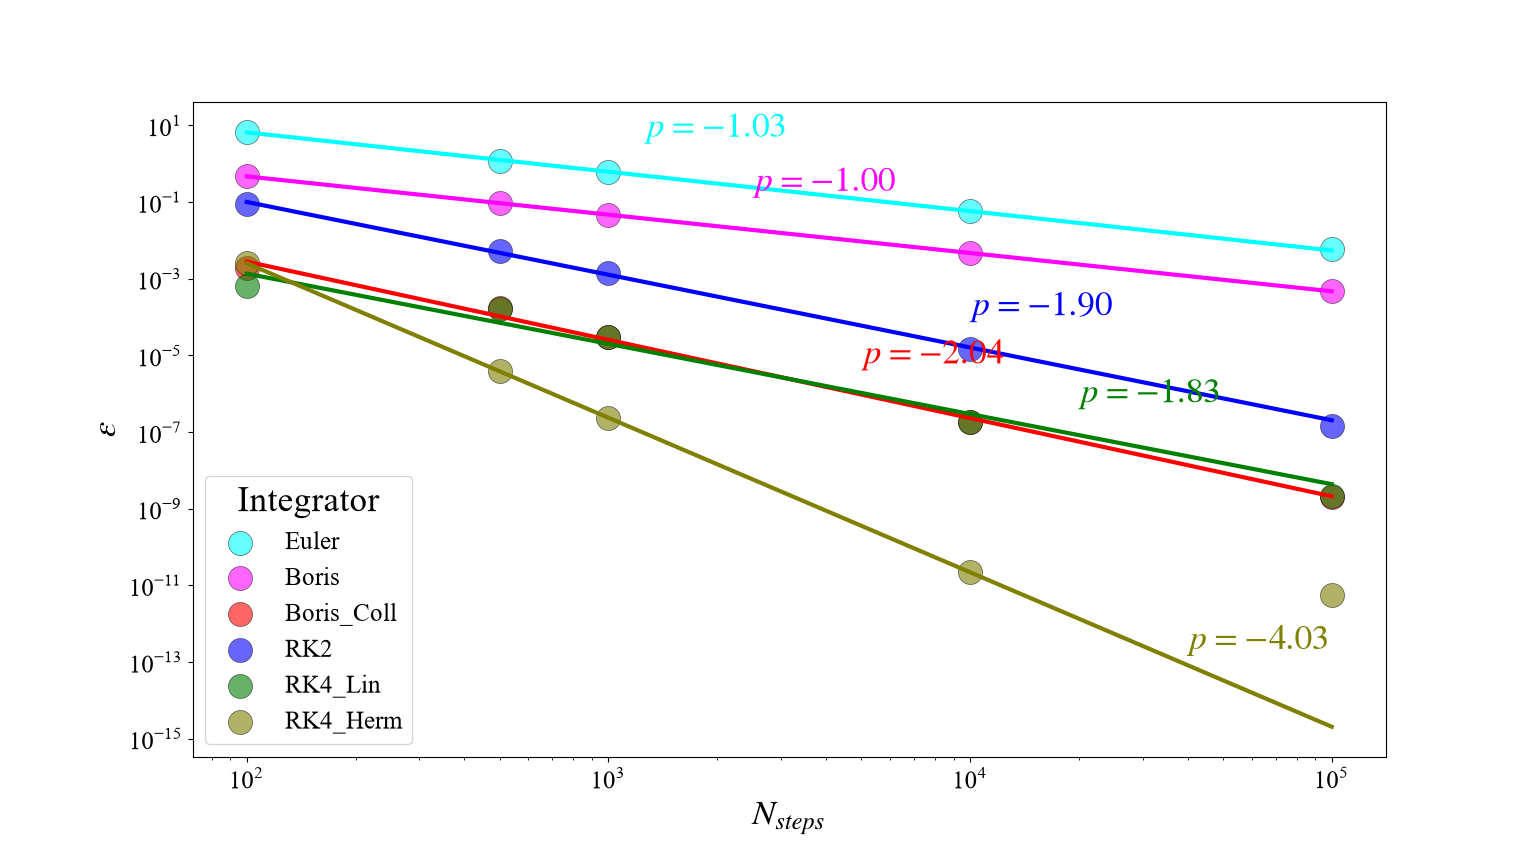
\includegraphics[width=0.82\textwidth]{Figures/Analitic solution/Conversion test/solvers vs analitic.png}
  \caption{Representative comparison of numerical integrators with the analytic solution.}
\end{figure}}{}

\IfFileExists{Figures/Analitic solution/Real Beam/Figure 1.png}{
\begin{figure}[H]
  \centering
  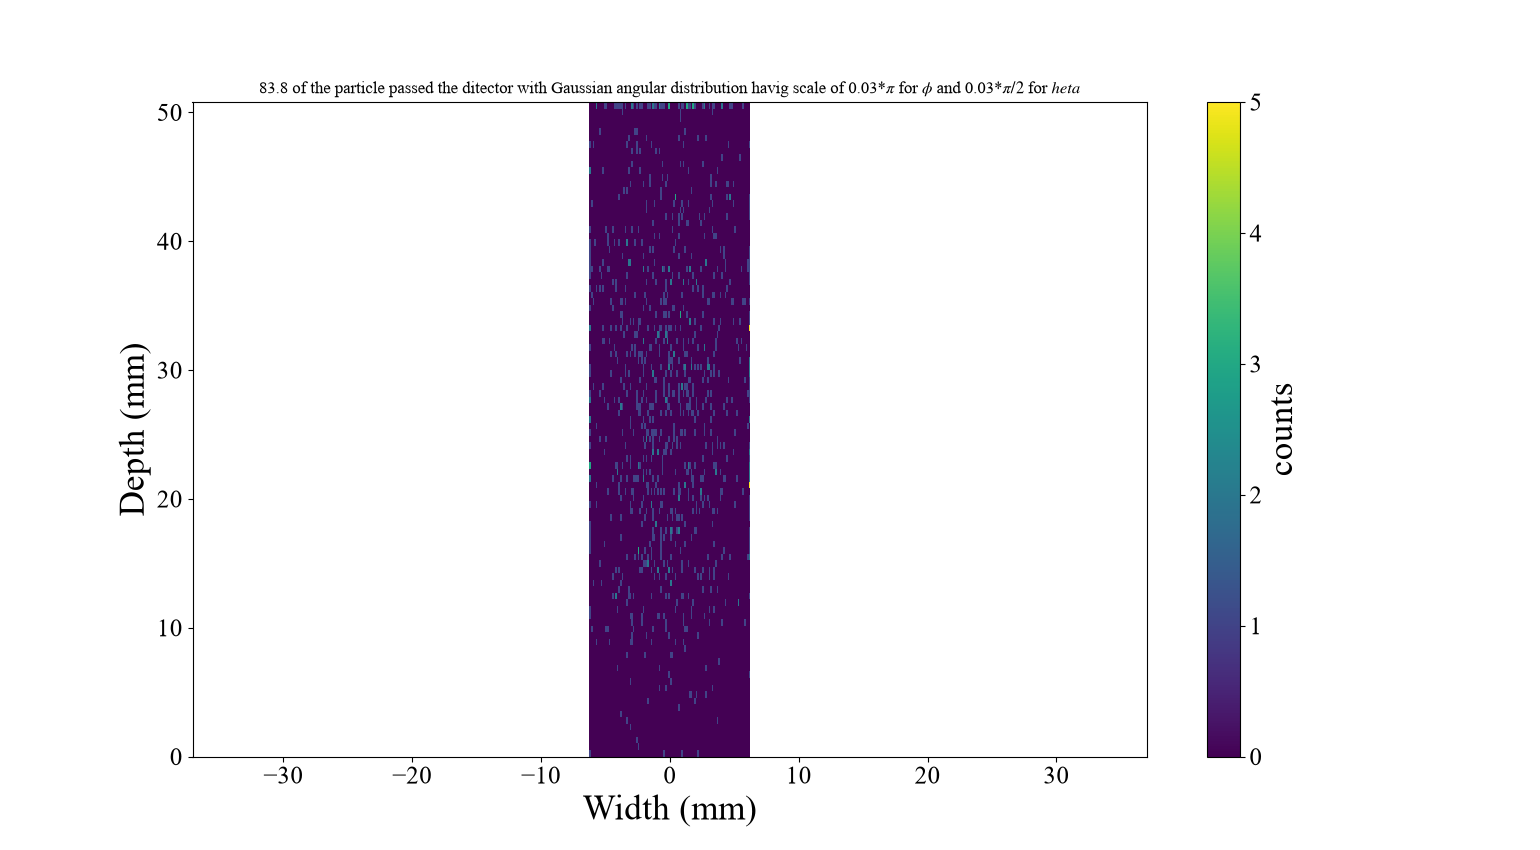
\includegraphics[width=0.82\textwidth]{Figures/Analitic solution/Real Beam/Figure 1.png}
  \caption{Representative synthetic real-beam detector distribution.}
\end{figure}}{}

\chapter{Validation Strategy}

A defensible validation sequence is:
\begin{enumerate}
  \item verify energy-to-velocity conversion and $\gamma$ reconstruction;
  \item compare the uniform-field exit position with
        \code{\_analitic\_sol\_vel2dist};
  \item verify expected time orders on the smooth analytic field;
  \item compare linear and spline field interpolation on a fixed numeric grid;
  \item verify magnetic-only speed or $\gamma$ conservation;
  \item refine the numeric potential grid separately from the time step;
  \item repeat stochastic beam runs with a fixed seed;
  \item record all geometry, species, field, grid, and time parameters with
        every final figure.
\end{enumerate}

Expected theoretical guidance is Euler order one, midpoint RK2 order two,
classical RK4 order four for a sufficiently smooth right-hand side, and Boris
order two when the field sampling and staggering are consistent.  Boundary
reconstruction and field interpolation can limit the observed order even when
the interior stepping formula has a higher formal order.

\chapter{Implementation Notes and Limitations}

\begin{itemize}
  \item The spelling \code{Analitic field}, \code{grid\_interpulation},
        \code{\_exect\_exist}, and \code{RK4\_Hermit} is part of the present
        program interface and must be used exactly unless the code is renamed
        consistently.
  \item The field model is built when \code{Integrators} is constructed or
        when \code{\_update\_solution} is called.  Updating the parameter
        dictionary alone does not regenerate a numeric potential.
  \item The spline clips query coordinates to its tabulated domain.  The
        numeric domain must therefore contain the complete trajectory region
        and fringe region of interest.
  \item Natural boundary conditions impose zero second derivative at the
        outer spline limits.  The computational field domain should extend
        far enough that this is a reasonable approximation.
  \item Cubic splines may overshoot near genuine discontinuities.  A physical
        Enge fringe is smooth, whereas an intentionally abrupt
        \code{fringe=0} field should not be interpreted as a smooth physical
        transition.
  \item The numeric field is based on a two-dimensional scalar-potential
        calculation and is not a general three-dimensional electromagnetic
        solver.
  \item Beam simulations can be memory- and CPU-intensive because integrator
        objects and field grids are copied into worker processes.
  \item Saved result figures are evidence of particular configurations; exact
        reproducibility additionally requires the parameter values, random
        seed, source version, and dependency versions.
\end{itemize}

\section{Maintenance checks}
When modifying the project, check the following paths together:
\begin{itemize}[noitemsep]
  \item both magnetic and electric interpolation paths;
  \item both analytic and numeric field construction branches;
  \item pinhole limits and body limits in every exit reconstruction method;
  \item scalar and array forms of energy input;
  \item single-process and multiprocessing execution;
  \item all enabled \code{if True} experiment blocks in \code{main.py}.
\end{itemize}

\chapter{Quick-Start Checklist}

\begin{enumerate}
  \item Install NumPy, Matplotlib, SciPy, and Joblib.
  \item Open \code{main.py} and set geometry, particle, and field parameters.
  \item Enable one field-initialization block.
  \item For numeric fields, select \code{"Linear"} or \code{"Spline"} and a
        $2^k+1$ grid.
  \item Enable the required experiment block and disable unrelated blocks.
  \item Rebuild the field after changing field-defining parameters.
  \item Run \code{python main.py} from the \code{Final} directory.
  \item Save the figure together with its parameter set and random seed.
  \item For convergence claims, inspect successive Richardson orders rather
        than relying only on one global fit.
\end{enumerate}

\appendix
\chapter{Minimal Programmatic Example}

\begin{lstlisting}
import numpy as np
from spectrometer.Experiment import Experiment
from spectrometer.integrators import Integrators

experiment = Experiment(
    height_mm=26,
    width_mm=12.5,
    depth_mm=50.8,
    shield_mm=5,
    yoke=0,
    pinhole_dia_mm=3,
    R0_mm=np.array([0.0, -10.0, 0.0]),
    q_eng_MeV=np.array([0.0, 3.0, 0.0]),
    m_kg=9.109e-31,
    q_C=-1.602e-19,
    Bx0_T=0.5,
    Ex0_Vm=0.0,
    fringe=1,
    sharp_edge=1,
    N_steps=1600,
    CFL=0.05,
    solution="Numeric Field",
    Nx_p=129,
    Ny_p=129,
    grid_interpulation="Spline",
)

params = experiment._evaluate_exp_paramas()
integrator = Integrators(params)
R_mm, v_ms, gamma = integrator._RK4_Hermit()
print("Exit position [mm]:", R_mm[-1])
\end{lstlisting}

\chapter{Natural Cubic Spline API}

\begin{lstlisting}
from spectrometer.custom_spline_2D import NaturalCubicSpline2D

# field.shape must be (len(y_axis), len(x_axis))
spline = NaturalCubicSpline2D(x_axis, y_axis, field)

# Scalar query -> scalar field-component value
field_at_particle = spline(x_particle, y_particle)

# Broadcast-compatible arrays -> array of field-component values
field_along_path = spline(x_positions, y_positions)
\end{lstlisting}

Internally, \code{P\_tag\_tag\_fun} solves for natural-spline second
derivatives and \code{Params\_finder} converts them to
$\alpha,\beta,\gamma,\eta$.  These functions are exposed primarily to make
the derivation transparent; normal simulation code should construct
\code{NaturalCubicSpline2D} and call the resulting object.

\end{document}
